\documentclass[12pt,a4paper,oneside]{article}

% ==========================================
% PACKAGES AND SETUP
% ==========================================
\usepackage[utf8]{inputenc}
\usepackage[T1]{fontenc}
\usepackage{lmodern}
\usepackage[margin=1in]{geometry}
\usepackage{amsmath,amssymb,amsthm,amsfonts,mathtools}
\usepackage{graphicx}
\usepackage{xcolor}
\usepackage{hyperref}
\usepackage{fancyhdr}
\usepackage{titlesec}
\usepackage{booktabs}
\usepackage{tikz}
\usetikzlibrary{arrows.meta,calc,decorations.markings,shapes,positioning}
\usepackage{setspace}
\usepackage{enumitem}
\usepackage{caption}
\usepackage{subcaption}

% Adjust headheight and margins to prevent header overlap warnings
\setlength{\headheight}{18pt}
\addtolength{\topmargin}{-6pt}

% ==========================================
% HYPERREF CONFIGURATION
% ==========================================
\hypersetup{
    colorlinks=true,
    linkcolor=navyblue,
    citecolor=teal,
    urlcolor=blue,
    pdftitle={UG Internship Report: Linear Dynamical Systems},
    pdfauthor={Chandramani Verma},
    pdfsubject={Linear Dynamical Systems, Annexure-3 Format},
    pdfkeywords={Dynamical Systems, Fundamental Theorem, Annexure-3, Banaras Hindu University}
}

% ==========================================
% COLOR DEFINITIONS
% ==========================================
\definecolor{navyblue}{RGB}{20, 40, 90}
\definecolor{darkteal}{RGB}{0, 100, 110}

% ==========================================
% THEOREM ENVIRONMENTS
% ==========================================
\theoremstyle{definition}
\newtheorem{definition}{Definition}[section]
\newtheorem{example}{Example}[section]
\newtheorem{remark}{Remark}[section]

\theoremstyle{plain}
\newtheorem{theorem}{Theorem}[section]
\newtheorem{lemma}[theorem]{Lemma}
\newtheorem{proposition}[theorem]{Proposition}
\newtheorem{corollary}[theorem]{Corollary}

% ==========================================
% HEADER & FOOTER SETUP
% ==========================================
\pagestyle{fancy}
\fancyhf{}
\fancyhead[L]{\small\nouppercase{Annexure-3: UG Internship Report}}
\fancyhead[R]{\small\thepage}
\renewcommand{\headrulewidth}{0.4pt}
\renewcommand{\footrulewidth}{0.4pt}
\fancyfoot[C]{\small Department of Mathematics $\cdot$ Banaras Hindu University}

% ==========================================
% SECTION TITLE FORMATTING
% ==========================================
\titleformat{\section}
  {\normalfont\Large\bfseries\color{navyblue}}{\thesection.}{0.8em}{}
\titleformat{\subsection}
  {\normalfont\large\bfseries\color{darkteal}}{\thesubsection}{0.8em}{}

\setstretch{1.58}

% ==========================================
% DOCUMENT BEGINS
% ==========================================
\begin{document}

% ------------------------------------------
% COVER & FRONT PAGE (ANNEXURE-3 FORMAT)
% ------------------------------------------
\begin{titlepage}
    \centering
    \vspace*{-0.5cm}
    
    
\includegraphics[height=3.6cm]{bhu_logo.png}\\[0.2cm]
    {\fontsize{18}{22}\selectfont \bfseries \color{navyblue} BANARAS HINDU UNIVERSITY\par}
    {\fontsize{11}{14}\selectfont \bfseries \color{darkteal} KASHI HINDU VISHWAVIDYALAYA $\cdot$ VARANASI -- 221005\par}
    
    \vspace{0.35cm}
    {\fontsize{13}{16}\selectfont \bfseries \color{navyblue} DEPARTMENT OF MATHEMATICS $\cdot$ INSTITUTE OF SCIENCE\par}
    
    \vspace{0.55cm}
    \rule{\linewidth}{1.5pt}
    \vspace{0.35cm}
    
    {\fontsize{16}{20}\selectfont \bfseries \color{navyblue} ANNEXURE-3\par}
    \vspace{0.18cm}
    {\fontsize{18}{22}\selectfont \bfseries \color{navyblue} UG INTERNSHIP REPORT\par}
    
    \vspace{0.45cm}
    {\fontsize{13}{17}\selectfont \bfseries TOPIC: LINEAR DYNAMICAL SYSTEMS\par}
    \vspace{0.25cm}
    {\fontsize{10}{14}\selectfont \itshape Module I: Preliminary Concepts, Autonomous and Non-Autonomous Systems, Diagonalization $\cdot$ Module II: Fundamental Theorem of Linear Systems $\cdot$ Module III: Jordan Canonical Forms, Stability Subspaces, Nonhomogeneous Systems\par}
    
    \vspace{0.35cm}
    \rule{\linewidth}{1.5pt}
    \vspace{0.55cm}
    
    % Annexure-3 Student Details Box
    \begin{center}
    \boldmath
    \begin{tabular}{|l l|}
        \hline
        \rule{0pt}{14pt}\textbf{Name of the Student:} & Chandramani Verma \\[0.2cm]
        \textbf{Enrollment No.:} & 474541 \\[0.2cm]
        \textbf{Examination Roll No.:} & 24220MAT063 \\[0.2cm]
        \textbf{Degree Program:} & Master of Science / Bachelor of Science in Mathematics \\[0.2cm]
        \textbf{Supervisor / Guide:} & Prof. Jai Prakash \\[0.2cm]
        \textbf{Date of Submission:} & July 25, 2026 \\[0.2cm]
        \hline
    \end{tabular}
    \end{center}

    \vfill
    
    \begin{center}
        \textbf{\large Department of Mathematics, Institute of Science}\\[0.1cm]
        \textbf{\large Banaras Hindu University, Varanasi -- 221005, Uttar Pradesh, India}\\[0.1cm]
        \textbf{\large Academic Session 2025--2026}
    \end{center}
\end{titlepage}

% ------------------------------------------
% PRELIMINARY PAGES (ACKNOWLEDGEMENTS & CONTENTS)
% ------------------------------------------
\newpage
\pagenumbering{roman}
\setcounter{page}{1}

% Acknowledgements
\section*{Acknowledgements}
\addcontentsline{toc}{section}{Acknowledgements}

I'm really grateful to my supervisor, \textbf{Prof. Jai Prakash} from the Department of Mathematics at BHU. He guided me throughout this 10-week internship. Whenever I got stuck on tough differential equation proofs, he patiently broke down the concepts until I understood them completely.

\vspace{0.35cm}
I'd also like to thank the Head of the Department and the Director of the Institute of Science for giving me access to the department library and study rooms. 

\vspace{0.25cm}
Thanks to my friends for the helpful group discussions, and to my family for always encouraging me during my studies.

\vspace{1.5cm}
\begin{flushright}
    \textbf{Chandramani Verma}\\
    Exam Roll No.: 24220MAT063\\
    Enrollment No.: 474541\\
    Department of Mathematics, Institute of Science\\
    Banaras Hindu University, Varanasi
\end{flushright}

\newpage
\tableofcontents

% ------------------------------------------
% MAIN CONTENT (ANNEXURE-3 SECTIONS)
% ------------------------------------------
\newpage
\pagenumbering{arabic}
\setcounter{page}{1}

% ==========================================
% SECTION 1: INTRODUCTION AND OBJECTIVE OF THE INTERNSHIP
% ==========================================
\section{Introduction and Objective of the Internship}
\label{sec:introduction}

\subsection{Preliminary Concepts and State Space}

\vspace{0.1cm}
Linear differential equations are everywhere in physics and engineering. Whether you're tracking spring vibrations or circuit currents, linear models give us a solid way to analyze system behavior. 

\smallskip
We write a standard continuous-time linear differential system in $n$-dimensional real space $\mathbb{R}^n$ as:
\begin{equation}
    \dot{x}(t) = A(t) x(t) + f(t), \quad x(t_0) = x_0
    \label{eq:state_space_general_human_v8}
\end{equation}
In this equation, $x(t) = (x_1(t), \dots, x_n(t))^T$ tracks the state vector at time $t$. The matrix $A(t)$ drives system dynamics, $f(t)$ handles external forces, and $x_0$ sets where the system starts at $t_0$.

\vspace{0.2cm}
Let's look at the basic geometry of phase space.

\begin{definition}[Phase Space and Trajectory]
The vector space $\mathbb{R}^n$ containing state vectors $x$ is called phase space. A curve $x(t)$ satisfying \eqref{eq:state_space_general_human_v8} is a solution trajectory starting from $x_0$. The function $v(t, x) = A(t)x + f(t)$ defines the vector field across $\mathbb{R}^n$.
\end{definition}

\medskip
\begin{definition}[Flow Operator]
When there's no forcing term ($\dot{x} = Ax$), the map $\phi_t(x_0) = e^{At} x_0$ is called the flow. It follows three simple rules:
\begin{enumerate}[label=(\alph*)]
    \item $\phi_0(x) = x$ (at time zero, nothing moves).
    \item $\phi_{t+s}(x) = \phi_t(\phi_s(x))$ (moving by $s$ then $t$ is the same as moving by $t+s$).
    \item $\phi_{-t} = (\phi_t)^{-1}$ (going backward in time undoes forward movement).
\end{enumerate}
\end{definition}

\subsection{Autonomous and Non-Autonomous Systems}

\vspace{0.15cm}
Linear systems fall into two main groups: autonomous and non-autonomous.

\smallskip
\begin{definition}[Autonomous System]
If $A$ doesn't change with time and $f(t) = 0$, the system is autonomous:
\begin{equation}
    \dot{x}(t) = A x(t), \quad x(0) = x_0
    \label{eq:autonomous_def_human_v8}
\end{equation}
Here, vector directions stay fixed in space. Shifting a solution in time gives another valid solution ($x(t - t_0)$). Because vector directions never change, two trajectories in an autonomous system can't cross each other in $\mathbb{R}^n$.
\end{definition}

\vspace{0.2cm}
\begin{definition}[Non-Autonomous System]
When $A(t)$ or $f(t)$ changes with time, the system is non-autonomous:
\begin{equation}
    \dot{x}(t) = A(t) x(t) + f(t), \quad x(t_0) = x_0
    \label{eq:nonautonomous_def_human_v8}
\end{equation}
Velocity vectors change as time passes. Trajectories passing through the same point at different times $t_1 \neq t_2$ take totally different paths.

To keep uniqueness, we work in extended space $\mathbb{R} \times \mathbb{R}^n$ with $\dot{t} = 1$.
\end{definition}

\vspace{0.3cm}
\begin{table}[htbp]
    \centering
    \caption{Comparison of Autonomous and Non-Autonomous Linear Systems}
    \label{tab:auto_nonauto_comparison_human_v8}
    \small
    \setstretch{1.3}
    \begin{tabular}{p{3.2cm} p{5.5cm} p{5.5cm}}
        \toprule
        \textbf{Property} & \textbf{Autonomous ($\dot{x}=Ax$)} & \textbf{Non-Autonomous ($\dot{x}=A(t)x+f(t)$)} \\
        \midrule
        Matrix $A$ & Constant matrix & Time-varying matrix $A(t)$ \\
        Flow Operator & Exponential map $\phi_t = e^{At}$ & Transition matrix $\Phi(t, t_0)$ \\
        Vector Field & Fixed over time & Changes with time $t$ \\
        State Solution & $x(t) = e^{At} x_0$ & Peano-Baker series / Variation of constants \\
        Fixed Points & Solutions to $Ax^* = 0$ & Time-dependent curves $x^*(t)$ \\
        Path Intersection & Can't cross in $\mathbb{R}^n$ & Can cross when projected onto $\mathbb{R}^n$ \\
        \bottomrule
    \end{tabular}
\end{table}

\subsection{Eigenspaces and Diagonalization}

\vspace{0.15cm}
Solutions to $\dot{x} = Ax$ depend directly on the eigenvalues and eigenvectors of $A$.

\begin{definition}[Eigenvalues and Eigenspace]
A scalar $\lambda \in \mathbb{C}$ is an eigenvalue of $A$ if $Av = \lambda v$ for some nonzero vector $v$. Eigenvalues are roots of $\det(\lambda I - A) = 0$. The subspace $E_\lambda = \ker(A - \lambda I)$ forms the eigenspace of $\lambda$.
\end{definition}

\begin{definition}[Diagonalization]
A matrix $A$ is diagonalizable if it has $n$ linearly independent eigenvectors $v_1, \dots, v_n$. Stacking them into $P = [v_1, \dots, v_n]$ gives $P^{-1} A P = D = \operatorname{diag}(\lambda_1, \dots, \lambda_n)$.
\end{definition}

\smallskip
Matrix trace $\operatorname{tr}(A) = \sum \lambda_i$ and determinant $\det(A) = \prod \lambda_i$ stay unchanged under basis transformations.

\subsection{Objectives of the Internship}

\vspace{0.15cm}
My internship focused on three core modules:
\begin{enumerate}[label=\arabic*.]
    \item \textbf{Module I:} Master state-space setup, vector fields, autonomous vs non-autonomous systems, and system decoupling through matrix diagonalization.
    \item \textbf{Module II:} Work through the Picard-Lindelöf existence-uniqueness proof, derive properties of $e^{At}$, and prove the Fundamental Theorem of Linear Systems.
    \item \textbf{Module III:} Study defective matrices, generalized eigenvectors, Jordan Canonical Forms, stability subspaces ($E^s, E^u, E^c$), 2D phase portraits, and Duhamel's formula for nonhomogeneous systems.
\end{enumerate}

% ==========================================
% SECTION 2: BRIEF DESCRIPTION OF INTERNSHIP ACTIVITIES
% ==========================================
\newpage
\section{Brief Description of Internship Activities}
\label{sec:activities}

\subsection{Module I Activities: Preliminary Concepts, Autonomous \& Non-Autonomous Systems, Diagonalization}

In Module I, I studied state-space models, flow properties, and decoupling linear systems into simpler scalar equations.

\subsubsection{1. Decoupling Systems by Linear Change of Variables}

\vspace{0.1cm}
Consider $\dot{x} = Ax$ where $A$ is diagonalizable ($A = P D P^{-1}$). Let's change variables using $x = P y$. Substituting this into our differential equation:
\begin{equation}
    P \dot{y} = A P y \implies \dot{y} = P^{-1} A P y = D y
\end{equation}
This breaks the original system into $n$ separate scalar differential equations:
\begin{align}
    \dot{y}_1 &= \lambda_1 y_1 \implies y_1(t) = e^{\lambda_1 t} y_1(0) \nonumber \\
    \dot{y}_2 &= \lambda_2 y_2 \implies y_2(t) = e^{\lambda_2 t} y_2(0) \nonumber \\
    &\vdots \nonumber \\
    \dot{y}_n &= \lambda_n y_n \implies y_n(t) = e^{\lambda_n t} y_n(0)
\end{align}
Transforming back to $x(t) = P y(t)$ gives:
\begin{equation}
    x(t) = P \operatorname{diag}(e^{\lambda_1 t}, \dots, e^{\lambda_n t}) P^{-1} x(0)
\end{equation}

\subsubsection{2. Picard-Lindelöf Theorem}

\vspace{0.15cm}
\begin{theorem}[Picard-Lindelöf Theorem]
If $A(t)$ and $f(t)$ are continuous on $[t_0, T]$, then $\dot{x}(t) = A(t)x(t) + f(t)$ with $x(t_0) = x_0$ has a unique solution on $[t_0, T]$.
\end{theorem}

\begin{proof}
Let $X = C([t_0, T], \mathbb{R}^n)$ with weighted norm $\|x\|_\lambda = \max_{t \in [t_0, T]} e^{-\lambda(t - t_0)} \|x(t)\|_2$. This space forms a complete Banach space.

Define the operator $\mathcal{T}: X \to X$ as:
\begin{equation}
    (\mathcal{T}x)(t) = x_0 + \int_{t_0}^t \left( A(s) x(s) + f(s) \right) ds
\end{equation}
For any two functions $x, y \in X$:
\begin{align}
    \|(\mathcal{T}x)(t) - (\mathcal{T}y)(t)\|_2 &\le \int_{t_0}^t \|A(s)\|_2 \|x(s) - y(s)\|_2 ds \nonumber \\
    &\le M \int_{t_0}^t e^{\lambda(s - t_0)} \|x - y\|_\lambda ds = M \|x - y\|_\lambda \frac{e^{\lambda(t - t_0)} - 1}{\lambda}
\end{align}
where $M = \max_{s \in [t_0, T]} \|A(s)\|_2$. Multiplying both sides by $e^{-\lambda(t - t_0)}$:
\begin{equation}
    \|\mathcal{T}x - \mathcal{T}y\|_\lambda \le \frac{M}{\lambda} \|x - y\|_\lambda
\end{equation}
Choosing $\lambda > M$ makes $\frac{M}{\lambda} < 1$. That means $\mathcal{T}$ is a contraction mapping. By Banach's fixed point theorem, $\mathcal{T}$ has one unique fixed point $x^*(t)$, which is our solution.
\end{proof}

\subsubsection{3. Grönwall's Inequality}

\vspace{0.15cm}
\begin{lemma}[Grönwall Inequality]
If $u(t) \le c + \int_{t_0}^t a(s) u(s) \, ds$ for continuous non-negative functions $u, a$ and constant $c \ge 0$, then $u(t) \le c \exp\left( \int_{t_0}^t a(s) \, ds \right)$.
\end{lemma}

\begin{proof}
Let $v(t) = c + \int_{t_0}^t a(s) u(s) ds$. Note that $v(t_0) = c$ and $u(t) \le v(t)$. Differentiating:
\begin{equation}
    \dot{v}(t) = a(t) u(t) \le a(t) v(t) \implies \dot{v}(t) - a(t) v(t) \le 0
\end{equation}
Multiply by integrating factor $\exp\left(-\int_{t_0}^t a(s) ds\right)$ to get $\frac{d}{dt}\left( v(t) \exp\left( -\int_{t_0}^t a(s) ds \right) \right) \le 0$. Integrating from $t_0$ to $t$ gives $v(t) \exp\left( -\int_{t_0}^t a(s) ds \right) \le c$, which means $u(t) \le c \exp\left( \int_{t_0}^t a(s) ds \right)$.
\end{proof}

\subsubsection{4. Floquet Theory for Periodic Systems}

\vspace{0.15cm}
When $A(t+T) = A(t)$ is periodic, Floquet theory shows the fundamental matrix factors into:
\begin{equation}
    \Phi(t) = P(t) e^{R t}
\end{equation}
where $P(t+T) = P(t)$ is periodic and $R$ is constant. Eigenvalues of $M = e^{RT}$ are Floquet multipliers. If all multipliers have magnitude $|\mu_j| < 1$, the periodic system is stable.

\subsubsection{5. Peano-Baker Series}

\vspace{0.15cm}
For non-autonomous systems $\dot{x} = A(t)x$ where $A(t)$ doesn't commute with itself at different times, the state transition matrix comes from the Peano-Baker series:
\begin{equation}
    \Phi(t, t_0) = I + \int_{t_0}^t A(s_1) \, ds_1 + \int_{t_0}^t A(s_1) \int_{t_0}^{s_1} A(s_2) \, ds_2 \, ds_1 + \dots
\end{equation}
This series converges uniformly and yields the solution $x(t) = \Phi(t, t_0) x_0$.

\subsection{Module II Activities: Fundamental Theorem of Linear Systems}

In Module II, I focused on matrix exponentials, proving uniform convergence, calculating derivatives, and establishing the fundamental theorem.

\subsubsection{1. Matrix Exponential Series}

\begin{definition}[Matrix Exponential]
For any square matrix $A \in \mathbb{R}^{n \times n}$ and real scalar $t$, $e^{At}$ is defined by the power series:
\begin{equation}
    e^{At} = \sum_{k=0}^{\infty} \frac{A^k t^k}{k!} = I + A t + \frac{A^2 t^2}{2!} + \dots
    \label{eq:matrix_exp_def_human_v8_6}
\end{equation}
\end{definition}

\begin{theorem}[Uniform Convergence]
For any $T > 0$, the series \eqref{eq:matrix_exp_def_human_v8_6} converges uniformly on $[-T, T]$.
\end{theorem}

\begin{proof}
Applying matrix norms:
\begin{equation}
    \left\| \sum_{k=0}^N \frac{A^k t^k}{k!} \right\| \le \sum_{k=0}^N \frac{\|A\|^k |t|^k}{k!} \le \sum_{k=0}^{\infty} \frac{(\|A\| T)^k}{k!} = e^{\|A\| T} < \infty
\end{equation}
By Weierstrass M-test, the matrix series converges uniformly on $[-T, T]$.
\end{proof}

\begin{lemma}[Derivative]
$\frac{d}{dt}(e^{At}) = A e^{At} = e^{At} A$.
\end{lemma}

\begin{proof}
Differentiating term by term:
\begin{equation}
    \frac{d}{dt}\left( \sum_{k=0}^{\infty} \frac{A^k t^k}{k!} \right) = \sum_{k=1}^{\infty} \frac{A^k k t^{k-1}}{k!} = A \sum_{m=0}^{\infty} \frac{A^m t^m}{m!} = A e^{At}
\end{equation}
\end{proof}

\subsubsection{2. Abel-Liouville-Jacobi Formula}

\vspace{0.15cm}
\begin{theorem}[Abel-Liouville-Jacobi Identity]
For any square matrix $A$, $\det(e^{At}) = e^{\operatorname{tr}(A) t}$.
\end{theorem}

\begin{proof}
For diagonalizable $A = P D P^{-1}$ with eigenvalues $\lambda_i$:
\begin{equation}
    \det(e^{At}) = \det(P e^{Dt} P^{-1}) = \det(e^{Dt}) = \prod e^{\lambda_i t} = e^{(\sum \lambda_i) t} = e^{\operatorname{tr}(A) t}
\end{equation}
Since diagonalizable matrices are dense in $\mathbb{R}^{n \times n}$, this identity holds for all square matrices.
\end{proof}

\subsubsection{3. Proof of Fundamental Theorem}

\vspace{0.15cm}
\begin{theorem}[Fundamental Theorem of Linear Systems]
The initial value problem $\dot{x}(t) = A x(t)$ with $x(0) = x_0$ has one unique solution $x(t) = e^{At} x_0$.
\end{theorem}

\begin{proof}
Existence: Differentiating $x(t) = e^{At} x_0$ gives $\dot{x}(t) = \frac{d}{dt}(e^{At}) x_0 = A e^{At} x_0 = A x(t)$, with initial value $x(0) = e^0 x_0 = x_0$.

Uniqueness: Suppose $y(t)$ is another solution. Let $z(t) = e^{-At} y(t)$. Differentiating:
\begin{equation}
    \dot{z}(t) = -A e^{-At} y(t) + e^{-At} \dot{y}(t) = -A e^{-At} y(t) + e^{-At} A y(t) = 0
\end{equation}
So $z(t)$ must be constant. Thus $z(t) = z(0) = x_0$, which means $y(t) = e^{At} x_0$.
\end{proof}

\subsubsection{4. Putzer's Algorithm}

\vspace{0.15cm}
\begin{theorem}[Putzer's Algorithm]
We can express $e^{At} = \sum_{k=0}^{n-1} r_{k+1}(t) P_k$ where $P_0 = I$, $P_k = \prod_{m=1}^k (A - \lambda_m I)$, and $r_k(t)$ are scalar functions defined by $\dot{r}_1 = \lambda_1 r_1$ ($r_1(0)=1$) and $\dot{r}_{k+1} = \lambda_{k+1} r_{k+1} + r_k$ ($r_{k+1}(0)=0$).
\end{theorem}

\subsection{Module III Activities: Jordan Canonical Forms, Stability Subspaces, Nonhomogeneous Systems}

In Module III, I covered defective matrices, generalized eigenvectors, Jordan forms, stability subspaces, and forced nonhomogeneous systems.

\subsubsection{1. Jordan Canonical Forms}

\vspace{0.15cm}
When an eigenvalue $\lambda$ has fewer independent eigenvectors than its algebraic multiplicity, matrix $A$ is defective and can't be diagonalized.

\begin{definition}[Generalized Eigenvector]
A nonzero vector $v$ is a generalized eigenvector of order $k$ for eigenvalue $\lambda$ if $(A - \lambda I)^k v = 0$ and $(A - \lambda I)^{k-1} v \neq 0$.
\end{definition}

\begin{theorem}[Jordan Canonical Form]
Any matrix $A$ is similar to a block diagonal matrix $J = P^{-1} A P = \operatorname{diag}(J_1(\lambda_1), \dots, J_m(\lambda_m))$ where Jordan blocks $J_k(\lambda)$ contain $\lambda$ on the main diagonal and ones right above it.
\end{theorem}

\subsubsection{2. Invariant Subspaces: Stable, Unstable, and Center Subspaces}

\vspace{0.15cm}
\begin{definition}[Invariant Subspaces]
Let eigenvalues of $A$ be $\lambda_j = \alpha_j + i \beta_j$.
\begin{enumerate}
    \item Stable Subspace ($E^s$): Spanned by generalized eigenvectors with $\operatorname{Re}(\lambda_j) < 0$. Solutions starting in $E^s$ decay to zero as $t \to \infty$.
    \item Unstable Subspace ($E^u$): Spanned by generalized eigenvectors with $\operatorname{Re}(\lambda_j) > 0$. Solutions starting in $E^u$ blow up to infinity as $t \to \infty$.
    \item Center Subspace ($E^c$): Spanned by generalized eigenvectors with $\operatorname{Re}(\lambda_j) = 0$. Solutions in $E^c$ oscillate or grow polynomially.
\end{enumerate}
\end{definition}

\begin{theorem}[Direct Sum Decomposition]
Phase space decomposes neatly into a direct sum: $\mathbb{R}^n = E^s \oplus E^u \oplus E^c$.
\end{theorem}

\begin{figure}[htbp]
    \centering
    \begin{tikzpicture}[scale=1.1, >=Stealth]
        % Axes / Subspace Planes
        \draw[thick, navyblue, ->] (-3.5, 0) -- (3.5, 0) node[right] {$E^s \text{ (Stable Subspace)}$};
        \draw[thick, darkteal, ->] (0, -3) -- (0, 3) node[above] {$E^u \text{ (Unstable Subspace)}$};
        
        % Trajectories in Stable Subspace (E^s)
        \draw[blue!80!black, thick, postaction={decorate, decoration={markings, mark=at position 0.6 with {\arrow{>}}}}] (3, 0) -- (0.1, 0);
        \draw[blue!80!black, thick, postaction={decorate, decoration={markings, mark=at position 0.6 with {\arrow{>}}}}] (-3, 0) -- (-0.1, 0);
        
        % Trajectories in Unstable Subspace (E^u)
        \draw[red!80!black, thick, postaction={decorate, decoration={markings, mark=at position 0.6 with {\arrow{>}}}}] (0, 0.1) -- (0, 2.8);
        \draw[red!80!black, thick, postaction={decorate, decoration={markings, mark=at position 0.6 with {\arrow{>}}}}] (0, -0.1) -- (0, -2.8);
        
        % Saddle Hyperbolic Curves
        \draw[purple, domain=0.4:3.0, samples=50, thick, postaction={decorate, decoration={markings, mark=at position 0.6 with {\arrow{>}}}}] plot ({\x}, {0.8/\x});
        \draw[purple, domain=-3.0:-0.4, samples=50, thick, postaction={decorate, decoration={markings, mark=at position 0.6 with {\arrow{>}}}}] plot ({\x}, {0.8/\x});
        \draw[purple, domain=0.4:3.0, samples=50, thick, postaction={decorate, decoration={markings, mark=at position 0.6 with {\arrow{>}}}}] plot ({\x}, {-0.8/\x});
        \draw[purple, domain=-3.0:-0.4, samples=50, thick, postaction={decorate, decoration={markings, mark=at position 0.6 with {\arrow{>}}}}] plot ({\x}, {-0.8/\x});

        % Origin Equilibrium
        \filldraw[black] (0,0) circle (3pt) node[below left] {$x^* = 0$};
    \end{tikzpicture}
    \caption{Phase portrait of a 2D saddle point showing stable ($E^s$) and unstable ($E^u$) invariant subspaces.}
    \label{fig:phase_portrait_subspaces_human_v8}
\end{figure}

\subsubsection{3. Classification of Planar Phase Portraits}

\vspace{0.15cm}
For a 2D system $\dot{x} = Ax$, phase portraits are classified using trace $\tau = \operatorname{tr}(A)$ and determinant $\Delta = \det(A)$:
\begin{itemize}
    \item Saddle Point: $\Delta < 0$.
    \item Stable Node: $\Delta > 0, \tau^2 \ge 4\Delta, \tau < 0$.
    \item Unstable Node: $\Delta > 0, \tau^2 \ge 4\Delta, \tau > 0$.
    \item Stable Focus: $\Delta > 0, \tau^2 < 4\Delta, \tau < 0$.
    \item Unstable Focus: $\Delta > 0, \tau^2 < 4\Delta, \tau > 0$.
    \item Center: $\Delta > 0, \tau = 0$.
\end{itemize}

\subsubsection{4. Nonhomogeneous Systems and Duhamel's Formula}

\vspace{0.15cm}
\begin{theorem}[Duhamel's Formula]
The general solution to $\dot{x}(t) = A x(t) + f(t)$ with $x(t_0) = x_0$ is:
\begin{equation}
    x(t) = e^{A(t - t_0)} x_0 + \int_{t_0}^t e^{A(t - s)} f(s) \, ds
    \label{eq:duhamel_constant_formula_human_v8}
\end{equation}
\end{theorem}

\begin{proof}
Set $x(t) = e^{At} v(t)$ where $v(0) = x_0$. Differentiating gives $\dot{x}(t) = A x(t) + e^{At} \dot{v}(t) = A x(t) + f(t) \implies \dot{v}(t) = e^{-At} f(t)$. Integrating from $0$ to $t$ gives $v(t) = x_0 + \int_0^t e^{-As} f(s) ds$. Multiplying through by $e^{At}$ yields equation \eqref{eq:duhamel_constant_formula_human_v8}.
\end{proof}

\subsection{Worked Examples}

\begin{example}[Planar System]
Find $e^{At}$ and $x(t)$ for $A = \begin{bmatrix} 1 & 2 \\ 0 & 3 \end{bmatrix}$ with initial state $x(0) = \begin{bmatrix} 2 \\ 1 \end{bmatrix}$.

\textbf{Solution:}
Characteristic equation $\det(\lambda I - A) = (\lambda - 1)(\lambda - 3) = 0$ gives eigenvalues $\lambda_1 = 1, \lambda_2 = 3$.
Corresponding eigenvectors are $v_1 = \begin{bmatrix} 1 \\ 0 \end{bmatrix}$ and $v_2 = \begin{bmatrix} 1 \\ 1 \end{bmatrix}$.
Constructing modal matrix and its inverse:
\begin{equation}
    P = \begin{bmatrix} 1 & 1 \\ 0 & 1 \end{bmatrix}, \quad P^{-1} = \begin{bmatrix} 1 & -1 \\ 0 & 1 \end{bmatrix}
\end{equation}
Calculating matrix exponential:
\begin{equation}
    e^{At} = P e^{Dt} P^{-1} = \begin{bmatrix} e^t & e^{3t} - e^t \\ 0 & e^{3t} \end{bmatrix}
\end{equation}
Multiplying by $x(0)$ gives the trajectory:
\begin{equation}
    x(t) = \begin{bmatrix} e^t & e^{3t} - e^t \\ 0 & e^{3t} \end{bmatrix} \begin{bmatrix} 2 \\ 1 \end{bmatrix} = \begin{bmatrix} e^t + e^{3t} \\ e^{3t} \end{bmatrix}
\end{equation}
\end{example}

\begin{example}[Nonhomogeneous System]
Solve $\dot{x}(t) = \begin{bmatrix} 0 & 1 \\ -2 & -3 \end{bmatrix} x(t) + \begin{bmatrix} 0 \\ e^{-t} \end{bmatrix}$ with initial condition $x(0) = \begin{bmatrix} 1 \\ 0 \end{bmatrix}$.

\textbf{Solution:}
For matrix $A = \begin{bmatrix} 0 & 1 \\ -2 & -3 \end{bmatrix}$, eigenvalues are $\lambda_1 = -1, \lambda_2 = -2$.
Eigenvectors $v_1 = \begin{bmatrix} 1 \\ -1 \end{bmatrix}$ and $v_2 = \begin{bmatrix} 1 \\ -2 \end{bmatrix}$.
$P = \begin{bmatrix} 1 & 1 \\ -1 & -2 \end{bmatrix}, P^{-1} = \begin{bmatrix} 2 & 1 \\ -1 & -1 \end{bmatrix}$.
Matrix exponential:
\begin{equation}
    e^{At} = \begin{bmatrix} 2e^{-t} - e^{-2t} & e^{-t} - e^{-2t} \\ -2e^{-t} + 2e^{-2t} & -e^{-t} + 2e^{-2t} \end{bmatrix}
\end{equation}
Homogeneous solution: $x_h(t) = e^{At} x(0) = \begin{bmatrix} 2e^{-t} - e^{-2t} \\ -2e^{-t} + 2e^{-2t} \end{bmatrix}$.
Particular integral via Duhamel:
\begin{equation}
    x_p(t) = \int_0^t \begin{bmatrix} e^{-(t-s)} - e^{-2(t-s)} \\ -e^{-(t-s)} + 2e^{-2(t-s)} \end{bmatrix} e^{-s} ds = \begin{bmatrix} t e^{-t} - e^{-t} + e^{-2t} \\ -t e^{-t} + 2e^{-t} - 2e^{-2t} \end{bmatrix}
\end{equation}
Adding homogeneous and particular parts gives $x(t) = \begin{bmatrix} (2 + t) e^{-t} \\ -(1 + t) e^{-t} \end{bmatrix}$.
\end{example}

\begin{example}[Defective Matrix]
Calculate $e^{At}$ for $A = \begin{bmatrix} 3 & 1 \\ 0 & 3 \end{bmatrix}$.

\textbf{Solution:}
Here $\lambda = 3$ is a repeated eigenvalue. We split $A = 3I + N$ where $N = \begin{bmatrix} 0 & 1 \\ 0 & 0 \end{bmatrix}$. Note that $N^2 = 0$.
Since $3I$ and $N$ commute:
\begin{equation}
    e^{At} = e^{3t} (I + Nt) = e^{3t} \begin{bmatrix} 1 & t \\ 0 & 1 \end{bmatrix} = \begin{bmatrix} e^{3t} & t e^{3t} \\ 0 & e^{3t} \end{bmatrix}
\end{equation}
\end{example}

\begin{example}[Harmonic Oscillator]
Find $e^{At}$ for $A = \begin{bmatrix} 0 & \omega \\ -\omega & 0 \end{bmatrix}$.

\textbf{Solution:}
Eigenvalues are complex conjugates $\lambda = \pm i \omega$. Summing the power series:
\begin{align}
    e^{At} &= I \left( 1 - \frac{\omega^2 t^2}{2!} + \dots \right) + \begin{bmatrix} 0 & 1 \\ -1 & 0 \end{bmatrix} \left( \omega t - \frac{\omega^3 t^3}{3!} + \dots \right) \nonumber \\
    &= \begin{bmatrix} \cos(\omega t) & \sin(\omega t) \\ -\sin(\omega t) & \cos(\omega t) \end{bmatrix}
\end{align}
\end{example}

\begin{example}[3D System]
Find $e^{At}$ for $A = \begin{bmatrix} -1 & 0 & 0 \\ 0 & 0 & 2 \\ 0 & -2 & 0 \end{bmatrix}$.

\textbf{Solution:}
Since $A$ is block diagonal:
\begin{equation}
    e^{At} = \begin{bmatrix} e^{-t} & 0 & 0 \\ 0 & \cos(2t) & \sin(2t) \\ 0 & -\sin(2t) & \cos(2t) \end{bmatrix}
\end{equation}
Stable subspace is $E^s = \operatorname{span}\{(1,0,0)^T\}$ and center subspace is $E^c = \operatorname{span}\{(0,1,0)^T, (0,0,1)^T\}$.
\end{example}

\begin{example}[4D System with Two Jordan Blocks]
Find $e^{Jt}$ for $J = \begin{bmatrix} 2 & 1 & 0 & 0 \\ 0 & 2 & 0 & 0 \\ 0 & 0 & -1 & 1 \\ 0 & 0 & 0 & -1 \end{bmatrix}$.

\textbf{Solution:}
Exponentiating the two separate Jordan blocks $J_1(2)$ and $J_2(-1)$:
\begin{equation}
    e^{Jt} = \begin{bmatrix} e^{2t} & t e^{2t} & 0 & 0 \\ 0 & e^{2t} & 0 & 0 \\ 0 & 0 & e^{-t} & t e^{-t} \\ 0 & 0 & 0 & e^{-t} \end{bmatrix}
\end{equation}
\end{example}

\begin{example}[Resonant Forced Oscillator]
Solve $\ddot{x} + \omega_0^2 x = \cos(\omega_0 t)$ with initial conditions $x(0) = 0, \dot{x}(0) = 0$.

\textbf{Solution:}
Writing in state-space form with $x_1 = x, x_2 = \dot{x}$:
\begin{equation}
    \begin{bmatrix} \dot{x}_1 \\ \dot{x}_2 \end{bmatrix} = \begin{bmatrix} 0 & 1 \\ -\omega_0^2 & 0 \end{bmatrix} \begin{bmatrix} x_1 \\ x_2 \end{bmatrix} + \begin{bmatrix} 0 \\ \cos(\omega_0 t) \end{bmatrix}
\end{equation}
Using Duhamel's integral gives $x_1(t) = \frac{t}{2\omega_0} \sin(\omega_0 t)$. The linear factor $t$ shows growing oscillations caused by resonance.
\end{example}

\subsection{Timeline of Internship Activities}

Table~\ref{tab:internship_activities_human_v8} summarizes the weekly work completed across the 10-week internship period.

\begin{table}[htbp]
    \centering
    \caption{Weekly Activities Schedule and Key Technical Deliverables}
    \label{tab:internship_activities_human_v8}
    \small
    \setstretch{1.3}
    \begin{tabular}{p{2.0cm} p{7.5cm} p{5.5cm}}
        \toprule
        \textbf{Timeline} & \textbf{Core Study Topics} & \textbf{Key Deliverables} \\
        \midrule
        Weeks 1--2 & Module I: State-space models, vector fields, autonomous vs non-autonomous systems & Formulated Section 1 definitions and comparative tables. \\
        Weeks 3--4 & Module I: Picard-Lindelöf theorem and contraction proofs & Verified existence/uniqueness proofs in function spaces. \\
        Weeks 5--6 & Module II: Matrix exponential $e^{At}$ properties and Fundamental Theorem & Proved $e^{At}$ uniform convergence and derivative formulas. \\
        Weeks 7--8 & Module III: Defective matrices, Jordan Canonical Forms, and invariant subspaces ($E^s, E^u, E^c$) & Computed JCF decompositions and drew phase portraits. \\
        Weeks 9--10 & Module III: Nonhomogeneous systems and Duhamel variation of parameters formula & Solved state trajectories for forced linear ODE systems. \\
        \bottomrule
    \end{tabular}
\end{table}

% ==========================================
% SECTION 3: CONCLUSION / KEY LEARNINGS OF INTERNSHIP
% ==========================================
\newpage
\section{Conclusion / Key Learnings of Internship}
\label{sec:conclusion}

This report highlights what I learned during my 10-week undergraduate internship on **Linear Dynamical Systems** under Prof. Jai Prakash at Banaras Hindu University, formatted according to **Annexure-3**.

\subsection{Summary of Learnings}

\vspace{0.15cm}
Working through these three modules gave me a solid grasp of linear system dynamics:
\begin{enumerate}[label=\arabic*.]
    \item \textbf{Module I Takeaways:} I gained a clear understanding of state-space models and vector fields. Studying autonomous systems showed me why solution curves in $\mathbb{R}^n$ don't cross. Proving Picard-Lindelöf theorem with Banach's fixed point theorem gave me a practical appreciation of how functional analysis guarantees unique differential equation solutions.
    \item \textbf{Module II Takeaways:} Working with matrix exponential $e^{At} = \sum_{k=0}^{\infty} \frac{A^k t^k}{k!}$ showed me how power series solve matrix differential equations. Proving uniform convergence with Weierstrass M-test and verifying $\frac{d}{dt}(e^{At}) = A e^{At}$ gave me the groundwork to prove the Fundamental Theorem of Linear Systems ($x(t) = e^{At} x_0$).
    \item \textbf{Module III Takeaways:} Handling defective matrices with chains of generalized eigenvectors showed me how to construct Jordan Canonical Forms when standard diagonalization fails. Decomposing phase space into stable ($E^s$), unstable ($E^u$), and center ($E^c$) subspaces made stability analysis straightforward. Finally, using Duhamel's formula helped me solve forced nonhomogeneous systems.
\end{enumerate}

\vspace{0.25cm}
Overall, this internship strengthened my knowledge of linear differential equations and matrix theory, giving me a solid foundation for future graduate work in applied mathematics.

% ==========================================
% REFERENCES
% ==========================================
\newpage
\renewcommand{\refname}{References}
\addcontentsline{toc}{section}{References}

\begin{thebibliography}{99}
    \bibitem{perko} L. Perko: \textit{Differential equations and dynamical systems}, Springer-Verlag, 2001.
    \bibitem{verhulst} F. Verhulst: \textit{Non-linear Differential Equations and Dynamical Systems}, Springer, 1990.
\end{thebibliography}

\end{document}
